\section{Why Wider Execution Changes the Reference}
\label{sec:reference}
\subsection{A masked suffix changes attention}
We begin with a CUDA Llama failure and locate the first numerical difference before analyzing its cause. The original reference processes continuation queries singly. At one four-query append, positions 765--768 require physical KV extents $[768,768,768,1024]$; an unsplit batch uses 1024 throughout. The first saved full target-vector difference occurs at generated-output index 29, whereas the first emitted-token difference occurs at index 81~\cite{records}. Inspecting only the divergent token would therefore start from a state that had already accumulated earlier discrepancies.

Captures at the first affected attention computation show identical visible Q, K, V, QK and softmax probability prefixes. The masked probability suffix is exactly zero. We then replay the native AV operator with captured operands, keeping the consumer query width at one. Cropping the wide execution's probability and V ranges to 768 reproduces the reference AV output. Padding the reference probability range with zeros and supplying the corresponding 1024-entry V range reproduces the wide output. Own-path replays reproduce their respective captures. These bidirectional interventions isolate the physical attention range as a numerical execution dependency (Fig.~\ref{fig:extent_intervention}).

\begin{figure*}[t]
\centering
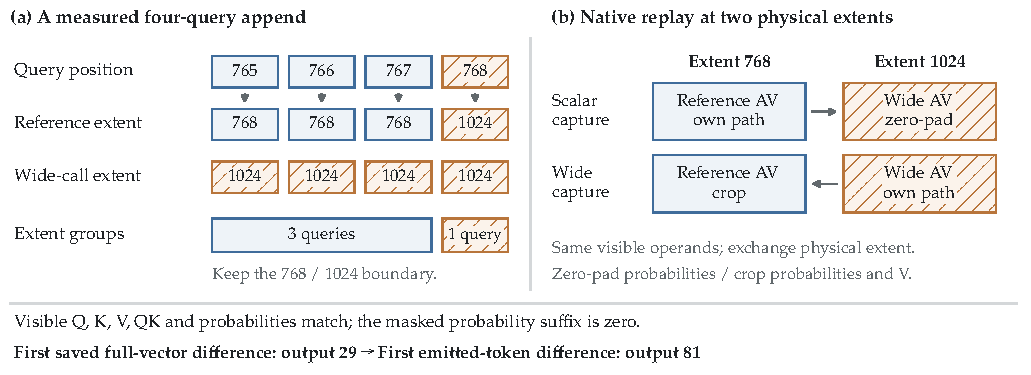
\includegraphics[width=\textwidth]{figures/extent_intervention.pdf}
\caption{Physical-range intervention on the CUDA Llama failure. The four queries require reference extents $[768,768,768,1024]$, while the unsplit call uses 1024. Replays of the first affected query exchange the cropped and padded AV ranges with the consumer query width fixed. The outputs follow the physical range despite identical visible operands and an exactly zero masked probability suffix. The first full-vector discrepancy precedes the first emitted-token discrepancy.}
\label{fig:extent_intervention}
\end{figure*}

The result explains why a logical mask alone cannot preserve this execution. The physical range is part of the native operator's descriptor even when some entries carry no attention mass. A Vulkan companion experiment reproduces the same kind of range dependency; there, changing the extent also changes contiguity and matvec dispatch. The required condition is therefore expressed in the backend's actual layout and execution terms.

\subsection{Query width selects arithmetic and placement}
The next question is whether matching the physical range suffices. Native projection experiments identify additional width-dependent choices. On an affected Vulkan Q8-weight path, a scalar operation consumes F32 activations, while a wider operation selects Q8\_1 activation quantization. Retaining the F32 path repairs that projection mismatch. In the Llama companion, this repair makes the emitted tokens agree while 99 committed full target vectors still differ. Applying the physical-prefix repair removes the remaining discrepancies~\cite{records}. Activation arithmetic and attention extent are separate requirements of the same execution.

On CUDA, the affected Q8 projection uses a small-column quantized matrix--vector (MMVQ) specialization. Traces for four and eight query columns show the same Q8\_1 input-quantizer kernel but different MMVQ launch organizations. Source inspection identifies four reduction warps at four columns and two at eight. Native replays with actual model operands match the scalar reference for the small-column path and diverge for the wider path~\cite{records}. This gives a useful unit of parallel work: preserve the four-column computation and expose several independent groups without selecting the eight-column reduction.

Placement is another part of that computation. In a partially offloaded Qwen deployment, increasing width moves K normalization and RoPE from CPU to CUDA. Replaying the same normalized K operands on the two placements makes the output follow placement; the input values alone do not explain the discrepancy~\cite{records}. A compatible implementation must retain the reference scheduling decision where it affects arithmetic. These experiments motivate a backend recipe that records activation types, reduction organization, placement, strides and dispatch conditions.

\subsection{Producer history and logical state connect the calls}
An arithmetic recipe operates on a state created by earlier phases. The prompt \emph{producer} is the execution that creates the incoming KV cache and initial target vector. In a controlled Vulkan experiment, exchanging the producer changes both the serialized KV and the complete initial target vector on all eight tested inputs. On two long inputs, either producer followed by scalar continuation reaches the reference token endpoint, but the parallel consumers reach that endpoint after only one producer~\cite{records}. Endpoint agreement by the producer and scalar consumer therefore does not establish that a later parallel phase begins from interchangeable numerical state.

The deployment's original producer must remain part of the execution. In our CUDA references it uses physical microbatch one with the original prompt caller and last-only output request. The resident Vulkan reference instead retains physical microbatch 128 and its declared outer prompt chunks. The continuation recipe can change at the phase boundary without replacing either producer.

State also has to survive the boundary \emph{after} a call. Verification may materialize several proposed tokens and retain only an accepted prefix. Its last physical output buffer can then belong to a rejected row, rather than to the retained frontier. A correction or bonus token can be emitted before it is materialized, and a generation cap or end-of-generation stop can leave that token pending. The executor must own requested vectors by logical row and update the active KV, frontier and pending-token record together. Otherwise, locally compatible arithmetic does not compose into a compatible request.

\subsection{The resulting execution target}
These observations define what is fixed before optimization. A deployment reference $R_d$ includes model and tokenizer bytes, formatting, numerical modules, device placement, KV type and capacity, producer calls, requested outputs, sampling and stopping behavior. The candidate $F_d$ changes the organization of known-query work under that reference.

For a materialized token prefix $x$, let $\ell^R(x)$ be its full binary32 target vocabulary vector and $K^R(x)$ its active KV in canonical logical order. The target relation at an observed state boundary is
\begin{equation}
 \ell^F(x)\bit\ell^R(x),\qquad K^F(x)\bit K^R(x),
 \label{eq:contract}
\end{equation}
together with matching logical positions, frontier, pending token and termination behavior. Equality compares complete values without a tolerance; unused storage is outside the active state.

Speculative verification also requests vectors on branches that may later be rejected. For each such vector, an independent reference follows the same prefix after the original producer. A separate autonomous reference supplies the emitted-token and stopping endpoint. The draft may propose different tokens; compatibility concerns the target computations on the prefixes actually evaluated. These observations make the execution requirements testable at both native-operator and complete-request levels.
